% --- ΚΕΦΑΛΑΙΟ 3: ΣΧΕΔΙΑΣΜΟΣ ΣΥΣΤΗΜΑΤΟΣ ---
\section{Σχεδιασμός Συστήματος}
\label{sec:sxediasmos_systimatos}
Το παρόν κεφάλαιο περιγράφει τον σχεδιασμό του εκπαιδευτικού λογισμικού.

\subsection{Αρχιτεκτονική}
\label{sec:arxitektoniki}
Η αρχιτεκτονική της εφαρμογής βασίζεται σε ένα σύγχρονο \eng{web stack}, συνδυάζοντας την ισχύ του \eng{Laravel framework} για το \eng{backend} και την ευελιξία του \eng{Vue.js} με το \eng{Inertia.js} για ένα δυναμικό \eng{frontend}.
\textbf{Βασικά Συστατικά Αρχιτεκτονικής:}
\begin{enumerate}[leftmargin=*, noitemsep]
    \item \textbf{\eng{Client} (Πελάτης - Φυλλομετρητής Ιστού):} Ο χρήστης αλληλεπιδρά με την εφαρμογή μέσω ενός φυλλομετρητή ιστού (\eng{web browser}). Το \eng{frontend}, χτισμένο με \eng{Vue.js}, είναι υπεύθυνο για την παρουσίαση της διεπαφής χρήστη (\eng{UI}) και την αρχική διαχείριση των αλληλεπιδράσεων.

    \item \textbf{\eng{Web Server \& Backend} Εφαρμογή (\eng{Laravel}):} Ένας \eng{web server}φιλοξενεί την \eng{backend} εφαρμογή που έχει αναπτυχθεί με το \eng{PHP framework Laravel}.
    \begin{itemize}[leftmargin=+, noitemsep]
        \item Το \eng{Laravel} ακολουθεί την αρχιτεκτονική \eng{Model-View-Controller (MVC)}:
        \begin{itemize}[leftmargin=++, noitemsep]
            \item \textbf{\eng{Models}:} Αντιπροσωπεύουν τη δομή των δεδομένων και την αλληλεπίδραση με τη βάση δεδομένων (π.χ. \eng{User, Course, Lesson, Quiz}).
            \item \textbf{\eng{Views}:} Σε αυτή την εφαρμογή, οι "\eng{Views}" του \eng{Laravel} δεν είναι παραδοσιακά \eng{Blade templates} που παράγουν \eng{HTML}. Αντ' αυτού, οι \eng{Controllers} επιστρέφουν απαντήσεις \eng{Inertia.js}, οι οποίες ουσιαστικά ενημερώνουν το \eng{frontend} ποιο \eng{Vue component} να φορτώσει και τι δεδομένα (\eng{props}) να του περάσει.
            \item \textbf{\eng{Controllers}:} Διαχειρίζονται τα αιτήματα του χρήστη, αλληλεπιδρούν με τα \eng{Models} για την ανάκτηση ή αποθήκευση δεδομένων, και επιστρέφουν την κατάλληλη απόκριση (\eng{Inertia response}) στο \eng{frontend}.
        \end{itemize}
        \item Το \eng{backend} είναι επίσης υπεύθυνο για την αυθεντικοποίηση των χρηστών, την εξουσιοδότηση, την επικύρωση των δεδομένων και τη συνολική επιχειρησιακή λογική της εφαρμογής.
    \end{itemize}

    \item \textbf{Βάση Δεδομένων:} Μια σχεσιακή βάση δεδομένων (\eng{SQLite}) χρησιμοποιείται για την αποθήκευση όλων των μόνιμων δεδομένων της εφαρμογής, όπως πληροφορίες χρηστών, περιεχόμενο μαθημάτων, πρόοδο χρηστών, και αποτελέσματα \eng{quiz}. Το \eng{Laravel Eloquent ORM} χρησιμοποιείται για την εύκολη αλληλεπίδραση με τη βάση δεδομένων.

    \item \textbf{\eng{Inertia.js}:} Το \eng{Inertia.js} λειτουργεί ως "κόλλα" μεταξύ του \eng{Laravel backend} και του \eng{Vue.js frontend}. Επιτρέπει την ανάπτυξη σύγχρονων, \eng{single-page application (SPA)} εμπειριών χωρίς την πολυπλοκότητα της δημιουργίας ενός ξεχωριστού \eng{API}. Όταν ο χρήστης πλοηγείται, το \eng{Inertia} κάνει αιτήματα \eng{XHR} στο \eng{backend}, και το \eng{backend} επιστρέφει \eng{JSON} που περιλαμβάνει το όνομα του \eng{Vue component} που πρέπει να φορτωθεί και τα δεδομένα (\eng{props}) που χρειάζεται. Το \eng{routing} γίνεται κυρίως από το \eng{Laravel}.
\end{enumerate}

\textbf{Ροή Δεδομένων (Υψηλού Επιπέδου):}
\begin{enumerate}[leftmargin=*, noitemsep]
    \item Ο χρήστης αλληλεπιδρά με το \eng{Vue.js component} στον \eng{browser} του (π.χ. κλικάρει ένα \eng{link} για ένα μάθημα).
    \item Το \eng{Inertia.js} υποβάλλει ένα αίτημα (\eng{request}) στον \eng{Laravel server}.
    \item Το αντίστοιχο \eng{Route} στο \eng{Laravel} ενεργοποιεί τον κατάλληλο \eng{Controller}.
    \item Ο \eng{Controller} επεξεργάζεται το αίτημα, αλληλεπιδρά με τα \eng{Models} για να πάρει δεδομένα από τη Βάση Δεδομένων.
    \item Ο \eng{Controller} επιστρέφει ένα \eng{Inertia Response}, το οποίο περιέχει το όνομα του \eng{Vue page component} και τα δεδομένα (\eng{props}) που χρειάζεται.
    \item Το \eng{Inertia.js} στο \eng{frontend} λαμβάνει την απάντηση, φορτώνει δυναμικά το νέο \eng{Vue component} (ή ενημερώνει το υπάρχον) με τα νέα \eng{props}, ενημερώνοντας το \eng{UI} χωρίς πλήρη επαναφόρτωση της σελίδας.
\end{enumerate}

\begin{figure}[h!]
  \centering
  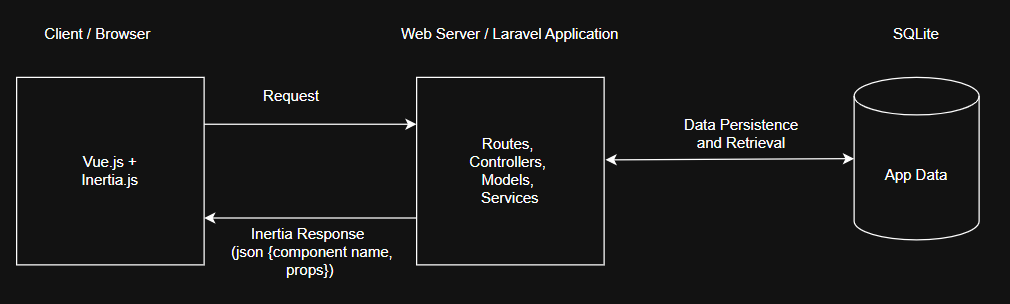
\includegraphics[scale=0.6]{architecture.png}
  \caption{Υψηλού Επιπέδου Αρχιτεκτονική Συστήματος.}
  \label{fig:arch_diag_placeholder_detailed}
\end{figure}

\subsection{Σχεδιασμός Βάσης Δεδομένων}
\label{sec:sxediasmos_bd_detailed}
Ο σχεδιασμός της βάσης δεδομένων αποτελεί θεμελιώδες τμήμα της εφαρμογής, καθώς είναι υπεύθυνος για την αποθήκευση και οργάνωση όλων των πληροφοριών που απαιτούνται για τη λειτουργία του εκπαιδευτικού λογισμικού. Χρησιμοποιήθηκε μια σχεσιακή βάση δεδομένων (\eng{SQLite} για την ανάπτυξη), και η αλληλεπίδραση με αυτήν γίνεται μέσω του \eng{Laravel Eloquent ORM}, το οποίο αντιστοιχίζει τους πίνακες της βάσης σε αντικείμενα (\eng{Models}).

Παρακάτω περιγράφονται οι κύριοι πίνακες (μοντέλα) της βάσης δεδομένων και οι μεταξύ τους σχέσεις.

\begin{figure}[h!]
  \centering
  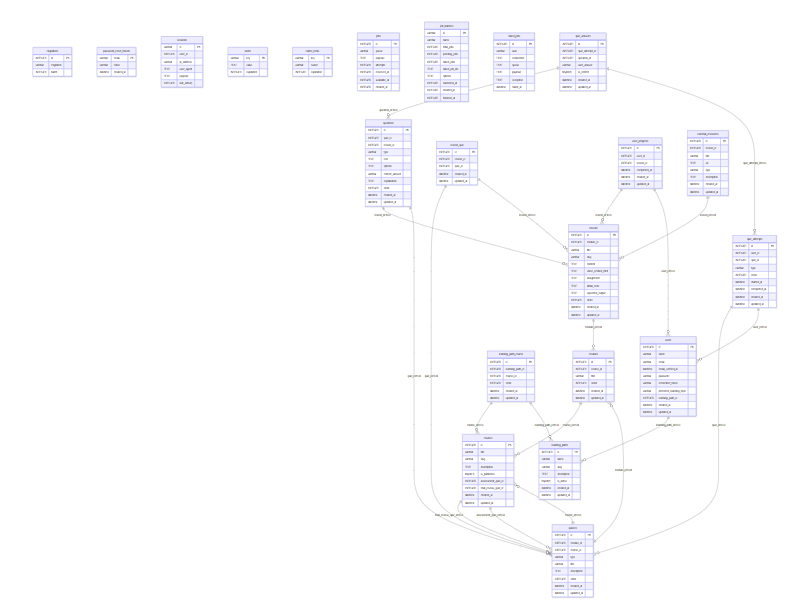
\includegraphics[scale=0.5]{erd.png}
  \caption{Διάγραμμα Σχήματος Βάσης Δεδομένων (\eng{ERD}).}
  \label{fig:erd_placeholder_detailed}
\end{figure}
\clearpage

\textbf{Περιγραφή Πινάκων (Μοντέλων):}

\begin{enumerate}[leftmargin=*, label=\arabic*., wide, labelwidth=!, labelindent=0pt, itemsep=1ex]
    \item \textbf{\texttt{\eng{users}} (Χρήστες):}
        \begin{itemize}[leftmargin=1.5em, noitemsep]
            \item \textit{Περιγραφή:} Αποθηκεύει πληροφορίες για τους εγγεγραμμένους χρήστες της πλατφόρμας.
            \item \textit{Βασικά Πεδία:} \texttt{\eng{id (PK)}}, \texttt{\eng{name}}, \texttt{\eng{email (unique)}}, \texttt{\eng{password (hashed)}}, \texttt{\eng{email\_verified\_at}}, \texttt{\eng{preferred\_learning\_style} (\eng{enum: 'reading', 'visual')}}, \texttt{\eng{learning\_path\_id (FK to learning\_paths, nullable)}}, \texttt{\eng{remember\_token}}, \texttt{\eng{timestamp}}.
            \item \textit{Σχέσεις:}
            \begin{itemize}[leftmargin=1.5em, noitemsep]
                \item Ένας χρήστης έχει πολλές εγγραφές προόδου (\eng{one-to-many with user\_progress}).
                \item Ένας χρήστης έχει πολλές προσπάθειες \eng{quiz (one-to-many with quiz\_attempts)}.
                \item Ένας χρήστης ανήκει σε μία μαθησιακή διαδρομή (\eng{many-to-one with learning\_paths}).
            \end{itemize}
        \end{itemize}

    \item \textbf{\texttt{\eng{learning\_paths}} (Μαθησιακές Διαδρομές):}
        \begin{itemize}[leftmargin=1.5em, noitemsep]
            \item \textit{Περιγραφή:} Καθορίζει προκαθορισμένες ακολουθίες μαθημάτων για συγκεκριμένους μαθησιακούς στόχους.
            \item \textit{Βασικά Πεδία:} \texttt{\eng{id (PK)}}, \texttt{\eng{name}}, \texttt{\eng{slug (unique)}}, \texttt{\eng{description}}, \texttt{\eng{is\_active}}, \texttt{\eng{timestamp}}.
            \item \textit{Σχέσεις:}
            \begin{itemize}[leftmargin=1.5em, noitemsep]
                \item Μία μαθησιακή διαδρομή έχει πολλούς χρήστες (\eng{one-to-many with users}).
                \item Μία μαθησιακή διαδρομή έχει πολλούς κύκλους μαθημάτων (\eng{many-to-many with courses} μέσω του πίνακα \texttt{\eng{learning\_path\_course}}).
            \end{itemize}
        \end{itemize}

    \item \textbf{\texttt{\eng{courses}} (Κύκλοι Μαθημάτων):}
        \begin{itemize}[leftmargin=1.5em, noitemsep]
            \item \textit{Περιγραφή:} Αντιπροσωπεύει ένα ολοκληρωμένο σύνολο διδακτικού υλικού για ένα ευρύτερο θέμα (π.χ., "\eng{JavaScript Fundamentals}").
            \item \textit{Βασικά Πεδία:} \texttt{\eng{id (PK)}}, \texttt{\eng{title}}, \texttt{\eng{slug (unique)}}, \texttt{\eng{description}}, \texttt{\eng{is\_published}}, \texttt{\eng{assessment\_quiz\_id} (\eng{FK} to \eng{quizzes, nullable})}, \texttt{\eng{final\_review\_quiz\_id (FK to quizzes, nullable)}}, \texttt{\eng{timestamp}}.
            \item \textit{Σχέσεις:}
            \begin{itemize}[leftmargin=1.5em, noitemsep]
                \item Ένας κύκλος μαθημάτων έχει πολλές ενότητες (\eng{one-to-many with modules}).
                \item Ένας κύκλος μαθημάτων ανήκει σε ένα (προαιρετικό) \eng{quiz} αξιολόγησης (\eng{many-to-one with quizzes}).
                \item Ένας κύκλος μαθημάτων ανήκει σε ένα (προαιρετικό) \eng{quiz} τελικής επανάληψης (\eng{many-to-one with quizzes}).
                \item Ένας κύκλος μαθημάτων ανήκει σε πολλές μαθησιακές διαδρομές (\eng{many-to-many with learning\_paths} μέσω του πίνακα \texttt{\eng{learning\_path\_course}}).
            \end{itemize}
        \end{itemize}

    \item \textbf{\texttt{\eng{modules}} (Ενότητες):}
        \begin{itemize}[leftmargin=1.5em, noitemsep]
            \item \textit{Περιγραφή:} Υποενότητες ενός \eng{Course}, ομαδοποιούν σχετικά μαθήματα.
            \item \textit{Βασικά Πεδία:} \texttt{\eng{id (PK)}}, \texttt{\eng{course\_id (FK)}}, \texttt{\eng{title}}, \texttt{\eng{order}}, \texttt{\eng{timestamp}}.
            \item \textit{Σχέσεις:}
            \begin{itemize}[leftmargin=1.5em, noitemsep]
                \item Μία ενότητα ανήκει σε έναν κύκλο μαθημάτων (\eng{many-to-one with courses}).
                \item Μία ενότητα έχει πολλά μαθήματα (\eng{one-to-many with lessons}).
                \item Μία ενότητα έχει πολλά \eng{quizzes (one-to-many with quizzes} - για τα \eng{module quizzes}).
            \end{itemize}
        \end{itemize}

    \item \textbf{\texttt{\eng{lessons}} (Μαθήματα):}
        \begin{itemize}[leftmargin=1.5em, noitemsep]
            \item \textit{Περιγραφή:} Η μικρότερη διδακτική μονάδα, περιέχει το εκπαιδευτικό υλικό και τις ασκήσεις.
            \item \textit{Βασικά Πεδία:} \texttt{\eng{id (PK)}}, \texttt{\eng{module\_id (FK)}}, \texttt{\eng{title}}, \texttt{\eng{slug (unique)}}, \texttt{\eng{content (HTML/Markdown)}}, \texttt{\eng{assignment}}, \texttt{\eng{initial\_code}}, \texttt{\eng{expected\_output}}, \texttt{\eng{video\_embed\_html (nullable)}}, \texttt{\eng{order}}, \texttt{\eng{timestamp}}.
            \item \textit{Σχέσεις:}
            \begin{itemize}[leftmargin=1.5em, noitemsep]
                \item Ένα μάθημα ανήκει σε μία ενότητα (\eng{many-to-one with modules}).
                \item Ένα μάθημα έχει πολλές εγγραφές προόδου χρηστών (\eng{one-to-many with user\_progress}).
                \item Ένα μάθημα έχει πολλές εξωτερικές πηγές (\eng{one-to-many with external\_resources}).
                \item Ένα μάθημα μπορεί να σχετίζεται με πολλές ερωτήσεις \eng{quiz (many-to-one from questions}).
            \end{itemize}
        \end{itemize}

    \item \textbf{\texttt{\eng{quizzes}}:}
        \begin{itemize}[leftmargin=1.5em, noitemsep]
            \item \textit{Περιγραφή:} Αντιπροσωπεύει ένα σύνολο ερωτήσεων για αξιολόγηση.
            \item \textit{Βασικά Πεδία:} \texttt{\eng{id (PK)}}, \texttt{\eng{type (enum: 'assessment', 'module', 'final\_review')}}, \texttt{\eng{module\_id (FK, nullable)}}, \texttt{\eng{title}}, \texttt{\eng{description}}, \texttt{\eng{order}}, \texttt{\eng{timestamp}}.
            \item \textit{Σχέσεις:}
            \begin{itemize}[leftmargin=1.5em, noitemsep]
                \item Ένα \eng{quiz} έχει πολλές ερωτήσεις (\eng{one-to-many with questions}).
                \item Ένα \eng{quiz} έχει πολλές προσπάθειες από χρήστες (\eng{one-to-many with quiz\_attempts}).
                \item Ένα \eng{quiz} (τύπου '\eng{module}') ανήκει σε μία ενότητα (\eng{many-to-one with modules}).
                \item Ένα \eng{quiz} (τύπου '\eng{assessment}' ή '\eng{final\_review}') μπορεί να συνδέεται με ένα \eng{course} (\eng{one-to-one relationships from courses}).
            \end{itemize}
        \end{itemize}

    \item \textbf{\texttt{\eng{questions}} (Ερωτήσεις):}
        \begin{itemize}[leftmargin=1.5em, noitemsep]
            \item \textit{Περιγραφή:} Μια μεμονωμένη ερώτηση ενός \eng{quiz}.
            \item \textit{Βασικά Πεδία:} \texttt{\eng{id (PK)}}, \texttt{\eng{quiz\_id (FK)}}, \texttt{\eng{lesson\_id (FK, nullable)}}, \texttt{\eng{type (enum: 'multiple\_choice', 'true\_false', 'fill\_blank')}}, \texttt{\eng{text}}, \texttt{\eng{options (JSON, nullable)}}, \texttt{\eng{correct\_answer}}, \texttt{\eng{explanation}}, \texttt{\eng{order}}, \texttt{\eng{timestamp}}.
            \item \textit{Σχέσεις:}
            \begin{itemize}[leftmargin=1.5em, noitemsep]
                \item Μία ερώτηση ανήκει σε ένα \eng{quiz (many-to-one with quizzes)}.
                \item Μία ερώτηση μπορεί να σχετίζεται με ένα μάθημα (\eng{many-to-one with lessons}).
            \end{itemize}
        \end{itemize}

    \item \textbf{\texttt{\eng{user\_progress}} (Πρόοδος Χρήστη):}
        \begin{itemize}[leftmargin=1.5em, noitemsep]
            \item \textit{Περιγραφή:} Καταγράφει την ολοκλήρωση μαθημάτων από τους χρήστες.
            \item \textit{Βασικά Πεδία:} \texttt{\eng{id (PK)}}, \texttt{\eng{user\_id (FK)}}, \texttt{\eng{lesson\_id (FK)}}, \texttt{\eng{completed\_at}}, \texttt{\eng{timestamp}}.
            \item \textit{Σχέσεις:}
            \begin{itemize}[leftmargin=1.5em, noitemsep]
                \item Ανήκει σε έναν χρήστη (\eng{many-to-one with users}).
                \item Ανήκει σε ένα μάθημα (\eng{many-to-one with lessons}).
            \end{itemize}
            \item \textit{Περιορισμός:} Μοναδικό ζεύγος (\texttt{\eng{user\_id, lesson\_id}}).
        \end{itemize}

    \item \textbf{\texttt{\eng{quiz\_attempts}} (Προσπάθειες \eng{Quiz}):}
        \begin{itemize}[leftmargin=1.5em, noitemsep]
            \item \textit{Περιγραφή:} Καταγράφει κάθε προσπάθεια ενός χρήστη σε ένα \eng{quiz}.
            \item \textit{Βασικά Πεδία:} \texttt{\eng{id (PK)}}, \texttt{\eng{user\_id (FK)}}, \texttt{\eng{quiz\_id (FK, nullable)}}, \texttt{\eng{type (string: 'standard', 'random', 'final\_review')}}, \texttt{\eng{score}}, \texttt{\eng{started\_at}}, \texttt{\eng{completed\_at}}, \texttt{\eng{timestamp}}.
            \item \textit{Σχέσεις:}
            \begin{itemize}[leftmargin=1.5em, noitemsep]
                \item Ανήκει σε έναν χρήστη (\eng{many-to-one with users}).
                \item Ανήκει σε ένα \eng{quiz (many-to-one with quizzes}, αν \texttt{quiz\_id not null}).
                \item Μία προσπάθεια έχει πολλές απαντήσεις (\eng{one-to-many with quiz\_answers}).
            \end{itemize}
        \end{itemize}

    \item \textbf{\texttt{\eng{quiz\_answers}} (Απαντήσεις \eng{Quiz}):}
        \begin{itemize}[leftmargin=1.5em, noitemsep]
            \item \textit{Περιγραφή:} Αποθηκεύει τη συγκεκριμένη απάντηση ενός χρήστη σε μια ερώτηση μιας προσπάθειας \eng{quiz}.
            \item \textit{Βασικά Πεδία:} \texttt{\eng{id (PK)}}, \texttt{\eng{quiz\_attempt\_id (FK)}}, \texttt{\eng{question\_id (FK)}}, \texttt{\eng{user\_answer}}, \texttt{\eng{is\_correct}}, \texttt{\eng{timestamp}}.
            \item \textit{Σχέσεις:}
            \begin{itemize}[leftmargin=1.5em, noitemsep]
                \item Ανήκει σε μία προσπάθεια \eng{quiz (many-to-one with quiz\_attempts)}.
                \item Ανήκει σε μία ερώτηση (\eng{many-to-one with questions}).
            \end{itemize}
            \item \textit{Περιορισμός:} Μοναδικό ζεύγος (\texttt{\eng{quiz\_attempt\_id, question\_id}}).
        \end{itemize}

    \item \textbf{\texttt{\eng{external\_resources}} (Εξωτερικές Πηγές):}
        \begin{itemize}[leftmargin=1.5em, noitemsep]
            \item \textit{Περιγραφή:} Σύνδεσμοι και πληροφορίες για επιπλέον υλικό μελέτης.
            \item \textit{Βασικά Πεδία:} \texttt{\eng{id (PK)}}, \texttt{\eng{lesson\_id (FK)}}, \texttt{\eng{title}}, \texttt{\eng{url}}, \texttt{\eng{type (enum)}}, \texttt{\eng{description}}, \texttt{\eng{timestamps}}.
            \item \textit{Σχέσεις:}
            \begin{itemize}[leftmargin=1.5em, noitemsep]
                \item Ανήκει σε ένα μάθημα (\eng{many-to-one with lessons}).
            \end{itemize}
        \end{itemize}

    \item \textbf{\texttt{\eng{learning\_path\_course}} (Πίνακας Συσχέτισης):}
        \begin{itemize}[leftmargin=1.5em, noitemsep]
            \item \textit{Περιγραφή:} Συνδέει τις μαθησιακές διαδρομές με τους κύκλους μαθημάτων, καθορίζοντας τη σειρά τους.
            \item \textit{Βασικά Πεδία:} \texttt{\eng{id (PK)}}, \texttt{\eng{learning\_path\_id (FK)}}, \texttt{\eng{course\_id (FK)}}, \texttt{\eng{order}}.
            \item \textit{Περιορισμός:} Μοναδικό ζεύγος (\texttt{\eng{learning\_path\_id, course\_id}}).
        \end{itemize}
\end{enumerate}

\subsection{Σχεδιασμός Λειτουργιών Εξατομίκευσης}
\label{sec:logiki_exatomikeusis}
Η εφαρμογή ενσωματώνει διάφορους μηχανισμούς για την παροχή μιας εξατομικευμένης μαθησιακής εμπειρίας. Ο σχεδιασμός αυτών των λειτουργιών βασίζεται στην ανάλυση των δεδομένων προόδου και των προτιμήσεων του χρήστη. Παρακάτω περιγράφεται η βασική λογική πίσω από κάθε χαρακτηριστικό εξατομίκευσης:

\begin{enumerate}[leftmargin=*, label=\arabic*., wide, labelwidth=!, labelindent=0pt, itemsep=1ex]
    \item \textbf{Πρόταση Παράκαμψης Μαθημάτων (\eng{Pre-course Assessment}):}
        \begin{itemize}[leftmargin=1.5em, noitemsep]
            \item \textit{Ενεργοποίηση:} Όταν ο χρήστης επιλέγει να ξεκινήσει ένα \eng{Course} που διαθέτει \eng{Quiz} Αξιολόγησης Αρχικού Επιπέδου (\texttt{\eng{assessment\_quiz}}).
            \item \textit{Διαδικασία:}
            \begin{enumerate}[leftmargin=1.5em, label=\alph*), noitemsep]
                \item Ο χρήστης ολοκληρώνει το \eng{Assessment Quiz}.
                \item Ο \texttt{\eng{CourseAssessmentController}} λαμβάνει τις απαντήσεις.
                \item Για κάθε ερώτηση του \eng{quiz} (οι οποίες είναι συνδεδεμένες με συγκεκριμένα αρχικά \eng{lessons} του \eng{Course} μέσω του πεδίου \texttt{\eng{lesson\_id}} στον πίνακα \texttt{\eng{questions}}), ελέγχεται η ορθότητα της απάντησης.
                \item Συγκεντρώνονται τα αποτελέσματα ανά \texttt{\eng{lesson\_id}}. Υπολογίζεται ένα ποσοστό επιτυχίας για τις ερωτήσεις που αντιστοιχούν σε κάθε αρχικό \eng{lesson}.
                \item Το σύστημα διατρέχει τα \eng{lessons} του \eng{Course} με τη σειρά.
                \item Εάν ένα \eng{lesson} δεν είχε ερωτήσεις στο \eng{assessment quiz}, ή εάν ο χρήστης δεν πέτυχε ένα προκαθορισμένο ποσοστό επιτυχίας (π.χ., 80\%) στις ερωτήσεις που αντιστοιχούσαν σε αυτό, τότε αυτό το \eng{lesson} προτείνεται ως το σημείο εκκίνησης.
                \item Εάν ο χρήστης περάσει επιτυχώς τις ερωτήσεις για όλα τα αρχικά \eng{lessons} που καλύπτονταν από το \eng{assessment}, του προτείνεται να ξεκινήσει από το πρώτο \eng{lesson} (ως ασφαλής επιλογή) ή ενημερώνεται ότι φαίνεται να κατέχει το υλικό και μπορεί να προχωρήσει σε πιο προχωρημένες ενότητες.
            \end{itemize}
            \item \textit{Αποτέλεσμα:} Ο χρήστης λαμβάνει μια προσωποποιημένη πρόταση για το από ποιο μάθημα θα μπορούσε να ξεκινήσει, μαζί με την επιλογή να αγνοήσει την πρόταση και να ξεκινήσει από την αρχή.
            \begin{figure}[h!]
              \centering
              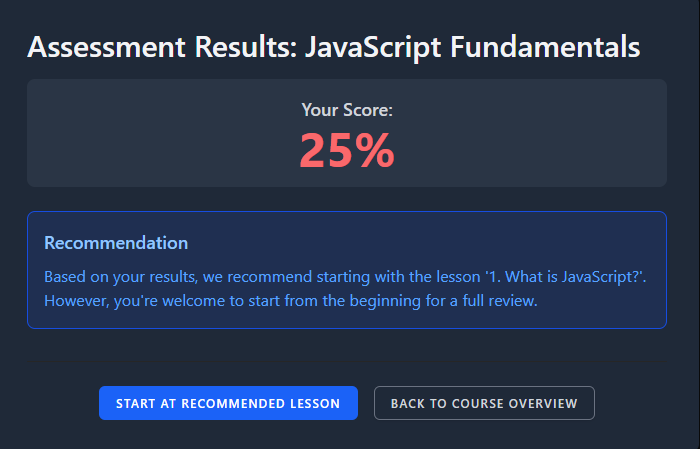
\includegraphics[scale=0.4]{images/assessment_result2.png}
              \caption{Πρόταση μαθήματος βάσει αξιολόγησης αρχικού επιπέδου.}
              \label{fig:pre_course_recom_placeholder}
            \end{figure}
        \end{itemize}

    \item \textbf{Πρόταση Ενισχυτικού Υλικού (\eng{Post-course Review Quiz}):}
        \begin{itemize}[leftmargin=1.5em, noitemsep]
            \item \textit{Ενεργοποίηση:} Μετά την ολοκλήρωση του Τελικού Επαναληπτικού \eng{Quiz} ενός \eng{Course}.
            \item \textit{Διαδικασία:}
            \begin{enumerate}[leftmargin=1.5em, label=\alph*), noitemsep]
                \item Ο χρήστης ολοκληρώνει το \eng{Post-course Review Quiz}.
                \item Ο \texttt{\eng{CourseReviewController}} λαμβάνει και βαθμολογεί τις απαντήσεις.
                \item Για κάθε λανθασμένη απάντηση, εντοπίζεται το \texttt{\eng{lesson\_id}} με το οποίο σχετίζεται η ερώτηση.
                \item Για κάθε τέτοιο \eng{lesson}, ανακτώνται από τη βάση δεδομένων οι σχετικές εξωτερικές πηγές υλικού (\texttt{\eng{external\_resources}}).
            \end{enumerate}
            \item \textit{Αποτέλεσμα:} Στη σελίδα αποτελεσμάτων του \eng{quiz}, μαζί με τις σωστές/λανθασμένες απαντήσεις, ο χρήστης βλέπει μια λίστα με τα μαθήματα που χρειάζονται επανάληψη και, για καθένα από αυτά, προτεινόμενους συνδέσμους προς εξωτερικές πηγές (άρθρα, βίντεο, τεκμηρίωση) για περαιτέρω μελέτη.
            \begin{figure}[h!]
              \centering
              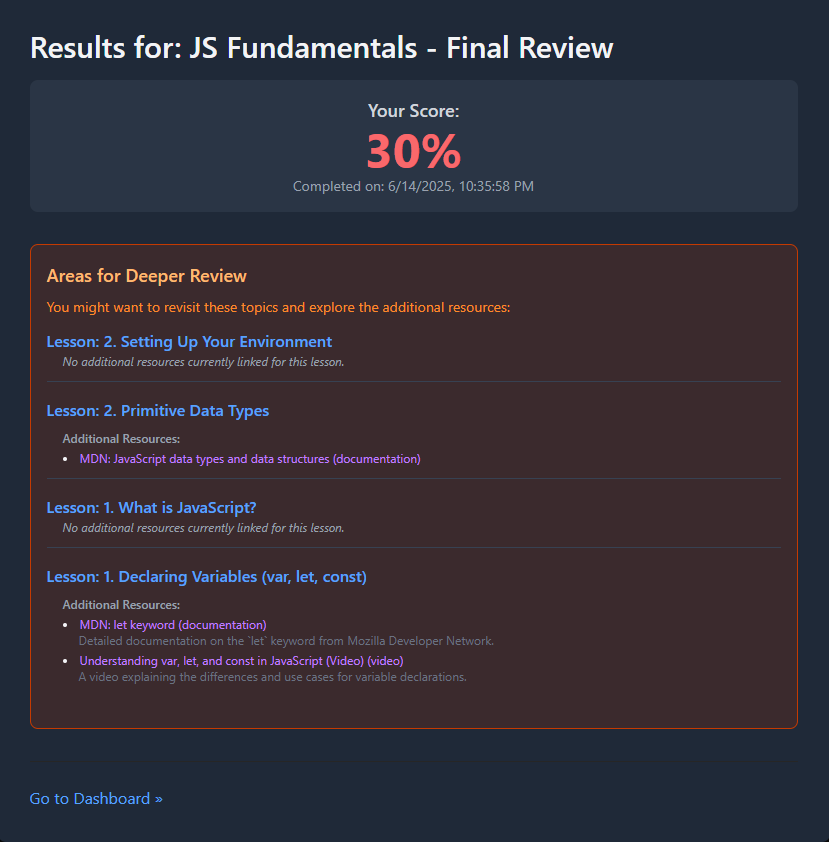
\includegraphics[scale=0.3]{images/final_review.png}
              \caption{Προτάσεις επανάληψης και ενισχυτικού υλικού.}
              \label{fig:post_course_resources_placeholder}
            \end{figure}
        \end{itemize}

    \item \textbf{Προσαρμογή Εμφάνισης Περιεχομένου (\eng{Visual vs. Reading Style}):}
        \begin{itemize}[leftmargin=1.5em, noitemsep]
            \item \textit{Ενεργοποίηση:} Ο χρήστης ορίζει την προτίμησή του (\texttt{\eng{preferred\_learning\_style}}) στο \eng{Dashboard}.
            \item \textit{Διαδικασία:}
            \begin{enumerate}[leftmargin=1.5em, label=\alph*), noitemsep]
                \item Η προτίμηση του χρήστη είναι διαθέσιμη στο \eng{frontend (Vue component lessons/Show.vue)} μέσω των \eng{global props} του \eng{Inertia}.
                \item Το \eng{component} ελέγχει την τιμή του \texttt{\eng{user.preferred\_learning\_style}} και την ύπαρξη ενσωματωμένου βίντεο (\texttt{\eng{lesson.video\_embed\_html}}).
                \item Εάν η προτίμηση είναι '\eng{visual}' και υπάρχει βίντεο, το μπλοκ του βίντεο εμφανίζεται πριν από το κειμενικό περιεχόμενο του μαθήματος.
                \item Σε αντίθετη περίπτωση (προτίμηση '\eng{reading}' ή δεν υπάρχει βίντεο), το κειμενικό περιεχόμενο εμφανίζεται πρώτο, και το βίντεο (αν υπάρχει) εμφανίζεται μετά, ως προαιρετικό.
            \end{enumerate}
            \item \textit{Αποτέλεσμα:} Η σειρά παρουσίασης των διαφορετικών τύπων περιεχομένου προσαρμόζεται στην προτίμηση του χρήστη, με στόχο την καλύτερη δυνατή εμπλοκή.
            \begin{figure}[h!]
              \centering
              
\includegraphics[scale=0.4]{images/visual_learner_lesson.png}
              \caption{Προσαρμογή εμφάνισης περιεχομένου.}
              \label{fig:lesson_visual_first_placeholder}
            \end{figure}
        \end{itemize}

    \item \textbf{Καθοδήγηση βάσει Μαθησιακού Στόχου (\eng{Learning Paths}):}
        \begin{itemize}[leftmargin=1.5em, noitemsep]
            \item \textit{Ενεργοποίηση:} Ο χρήστης επιλέγει μια Μαθησιακή Διαδρομή (\texttt{\eng{learning\_path}}) στο \eng{Dashboard}.
            \item \textit{Διαδικασία:}
            \begin{enumerate}[leftmargin=1.5em, label=\alph*), noitemsep]
                \item Η επιλεγμένη διαδρομή του χρήστη είναι γνωστή στο \eng{backend (DashboardController)}.
                \item Ο \eng{controller} ανακτά τα \eng{Courses} που ανήκουν σε αυτή τη διαδρομή, στη σωστή σειρά (βάσει του πεδίου \texttt{order} στον πίνακα \texttt{\eng{learning\_path\_course}}).
                \item Για κάθε \eng{Course} στη διαδρομή, ελέγχεται η πρόοδος του χρήστη (ολοκληρωμένα \eng{lessons} μέσω του \texttt{\eng{user\_progress}}).
                \item Το πρώτο \eng{Course} στη σειρά της διαδρομής για το οποίο ο χρήστης δεν έχει ολοκληρώσει όλα τα μαθήματα (ή ένα σημαντικό ποσοστό αυτών) προτείνεται ως το "Επόμενο Προτεινόμενο \eng{Course}".
                \item Αν όλα τα \eng{Courses} της διαδρομής έχουν ολοκληρωθεί, εμφανίζεται ένα μήνυμα επιτυχίας.
            \end{enumerate}
            \item \textit{Αποτέλεσμα:} Στο \eng{Dashboard}, ο χρήστης βλέπει την τρέχουσα μαθησιακή του διαδρομή και μια σαφή πρόταση για το ποιο \eng{course} να παρακολουθήσει στη συνέχεια, παρέχοντας δομή και κατεύθυνση.
            \begin{figure}[h!]
              \centering
              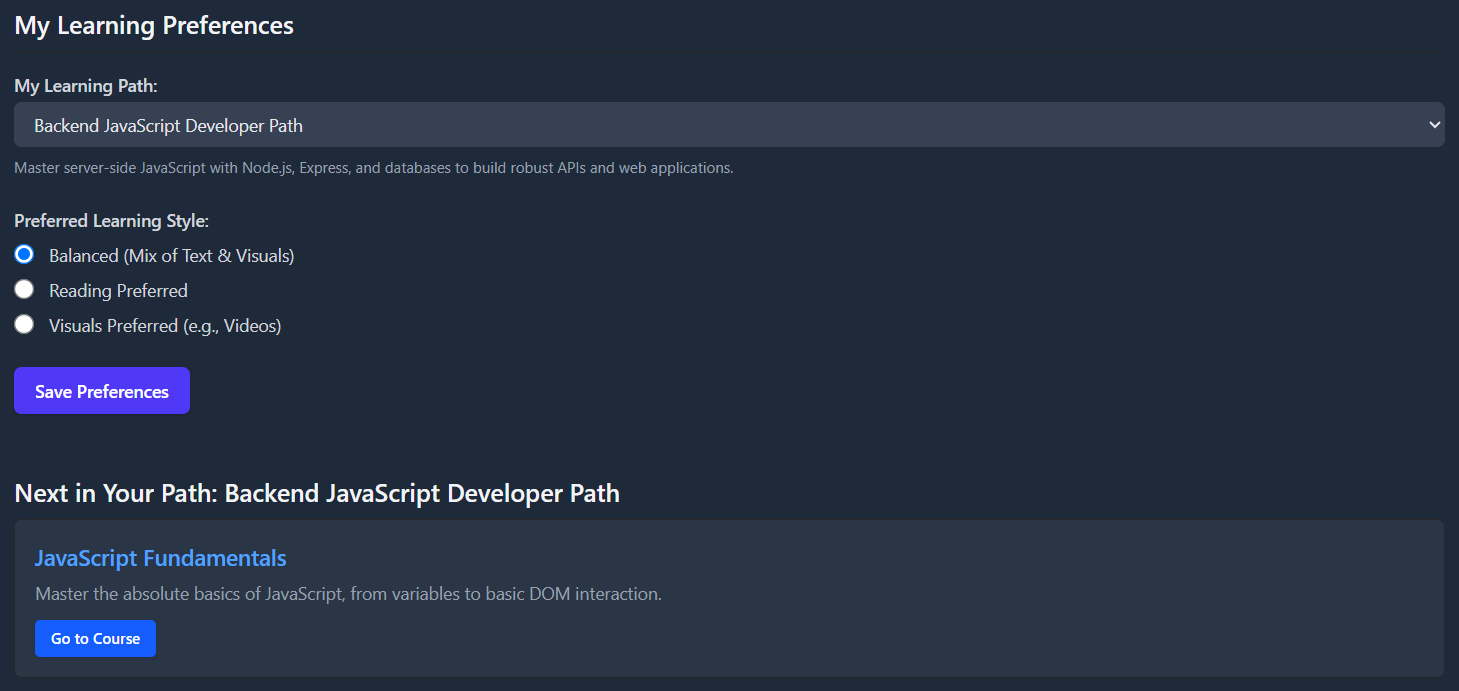
\includegraphics[scale=0.3]{images/learning_path.png}
              \caption{Καθοδήγηση μαθησιακής διαδρομής.}
              \label{fig:dashboard_path_suggestion_placeholder}
            \end{figure}
        \end{itemize}
\end{enumerate}

\subsection{Σημαντικά \eng{Components}}
\label{sec:simantika_components_detailed}
Η εφαρμογή δομείται γύρω από ένα σύνολο διακριτών \eng{components} στο \eng{backend} (κυρίως \eng{Laravel Controllers}) και στο \eng{frontend} (\eng{Vue Pages} και επαναχρησιμοποιήσιμα \eng{Vue Components}). Αυτή η προσέγγιση προάγει την οργάνωση, τη συντηρησιμότητα και την επεκτασιμότητα του κώδικα.

\subsubsection{\eng{Backend Components (Laravel Controllers)}}
\label{sec:backend_controllers_detailed}
Οι παρακάτω είναι οι κύριοι \eng{controllers} που διαχειρίζονται την επιχειρησιακή λογική της εφαρμογής στην πλευρά του \eng{server}:
\begin{itemize}[leftmargin=*, noitemsep]
    \item \textbf{\texttt{\eng{DashboardController}}:}
        \begin{itemize}[leftmargin=+, noitemsep]
            \item \textit{Ρόλος:} Υπεύθυνος για τη συγκέντρωση και παροχή των δεδομένων που απαιτούνται για την αρχική σελίδα (\eng{dashboard}) του συνδεδεμένου χρήστη. Αυτό περιλαμβάνει τις προτιμήσεις του χρήστη (\eng{learning path, learning style}), τις διαθέσιμες μαθησιακές διαδρομές, το επόμενο προτεινόμενο \eng{course} βάσει της επιλεγμένης διαδρομής, και το ιστορικό πρόσφατων προσπαθειών σε \eng{quizzes}.
        \end{itemize}
    \item \textbf{\texttt{\eng{CourseController}}:}
        \begin{itemize}[leftmargin=+, noitemsep]
            \item \textit{Ρόλος:} Διαχειρίζεται τις λειτουργίες που σχετίζονται με τους κύκλους μαθημάτων (\eng{Courses}).
            \item \textit{Βασικές Μέθοδοι:} \texttt{\eng{index()}} για την εμφάνιση λίστας όλων των δημοσιευμένων \eng{courses}, \texttt{\eng{show()}} για την εμφάνιση των λεπτομερειών ενός συγκεκριμένου \eng{course (modules, lessons, quizzes} ενότητας, \eng{link} για \eng{assessment/review}).
        \end{itemize}
    \item \textbf{\texttt{\eng{LessonController}}:}
        \begin{itemize}[leftmargin=+, noitemsep]
            \item \textit{Ρόλος:} Διαχειρίζεται την εμφάνιση των μεμονωμένων μαθημάτων (\eng{Lessons}).
            \item \textit{Βασικές Μέθοδοι:} \texttt{\eng{show()}} для την παρουσίαση του περιεχομένου ενός μαθήματος, της άσκησης, του αρχικού κώδικα και την προετοιμασία της διεπαφής με τον \eng{code editor}.
        \end{itemize}
    \item \textbf{\texttt{\eng{QuizController}}:}
        \begin{itemize}[leftmargin=+, noitemsep]
            \item \textit{Ρόλος:} Διαχειρίζεται τη διεξαγωγή των τυπικών \eng{quizzes (module quizzes)}.
            \item \textit{Βασικές Μέθοδοι:} \texttt{\eng{show()}} для την εμφάνιση των ερωτήσεων ενός \eng{quiz}, \texttt{\eng{submit()}} для την παραλαβή των απαντήσεων, τη βαθμολόγηση, την αποθήκευση της προσπάθειας (\eng{QuizAttempt} και \eng{QuizAnswer}) και την εμφάνιση των αποτελεσμάτων.
        \end{itemize}
    \item \textbf{\texttt{\eng{UserProgressController}}:}
        \begin{itemize}[leftmargin=+, noitemsep]
            \item \textit{Ρόλος:} Διαχειρίζεται την καταγραφή της προόδου του χρήστη.
            \item \textit{Βασικές Μέθοδοι:} \texttt{\eng{store()}} для την επισήμανση ενός μαθήματος (\eng{Lesson}) ως ολοκληρωμένου από τον χρήστη, συνήθως μετά την επιτυχή ολοκλήρωση της άσκησης κώδικα.
        \end{itemize}
    \item \textbf{\texttt{\eng{CourseAssessmentController}}:}
        \begin{itemize}[leftmargin=+, noitemsep]
            \item \textit{Ρόλος:} Διαχειρίζεται τα \eng{quizzes} αξιολόγησης αρχικού επιπέδου (\eng{Pre-course Assessment}).
            \item \textit{Βασικές Μέθοδοι:} \texttt{\eng{show()}} για την εμφάνιση του \eng{assessment quiz}, \texttt{\eng{submit()}} για τη βαθμολόγηση και την παροχή πρότασης σχετικά με το από ποιο μάθημα να ξεκινήσει ο χρήστης.
        \end{itemize}
    \item \textbf{\texttt{\eng{CourseReviewController}}:}
        \begin{itemize}[leftmargin=+, noitemsep]
            \item \textit{Ρόλος:} Διαχειρίζεται τα τελικά επαναληπτικά \eng{quizzes} ενός \eng{course (Post-course Review)}.
            \item \textit{Βασικές Μέθοδοι:} \texttt{\eng{generate()}} για τη δυναμική δημιουργία του \eng{quiz} (βάσει προηγούμενων λανθασμένων απαντήσεων και νέων ερωτήσεων), \texttt{\eng{submit()}} για τη βαθμολόγηση, την αποθήκευση της προσπάθειας και την παροχή προτάσεων για επανάληψη μαθημάτων και εξωτερικών πηγών.
        \end{itemize}
    \item \textbf{\texttt{\eng{RandomQuizController}}:}
        \begin{itemize}[leftmargin=+, noitemsep]
            \item \textit{Ρόλος:} Διαχειρίζεται τη δημιουργία και διεξαγωγή τυχαίων \eng{quizzes} επανάληψης.
            \item \textit{Βασικές Μέθοδοι:} \texttt{\eng{generate()}} για την επιλογή τυχαίων ερωτήσεων από τα ολοκληρωμένα μαθήματα του χρήστη, \texttt{\eng{submit()}} για τη βαθμολόγηση και την αποθήκευση της προσπάθειας.
        \end{itemize}
    \item \textbf{\texttt{\eng{UserPreferenceController}}:}
        \begin{itemize}[leftmargin=+, noitemsep]
            \item \textit{Ρόλος:} Διαχειρίζεται την ενημέρωση των μαθησιακών προτιμήσεων του χρήστη (\eng{learning style, learning path}) από το \eng{Dashboard}.
            \item \textit{Βασικές Μέθοδοι:} \texttt{\eng{update()}} για την αποθήκευση των νέων προτιμήσεων.
        \end{itemize}
    \item \textbf{\texttt{\eng{UserStatsController}}:}
        \begin{itemize}[leftmargin=+, noitemsep]
            \item \textit{Ρόλος:} Συγκεντρώνει και παρέχει τα δεδομένα για τη σελίδα στατιστικών του χρήστη.
            \item \textit{Βασικές Μέθοδοι:} \texttt{\eng{show()}} για την προετοιμασία των δεδομένων (\eng{learning streak}, κατανομή σκορ \eng{quiz}, δεδομένα για \eng{contribution graph}).
        \end{itemize}
    \item \textbf{\texttt{\eng{ProfileController}}:}
        \begin{itemize}[leftmargin=+, noitemsep]
            \item \textit{Ρόλος:} Διαχειρίζεται τις βασικές λειτουργίες προφίλ χρήστη (επεξεργασία ονόματος, \eng{email, password}). Η λειτουργικότητα για τις μαθησιακές προτιμήσεις μεταφέρθηκε στο \eng{DashboardController} και \eng{UserPreferenceController} για ευκολότερη πρόσβαση από τον χρήστη.
        \end{itemize}
\end{itemize}

\subsubsection{\eng{Frontend Components (Vue Pages \&} Κύρια \eng{Components)}}
\label{sec:frontend_components_detailed}
Η διεπαφή χρήστη (\eng{UI}) υλοποιείται με \eng{Vue.js} και \eng{Inertia.js}. Οι παρακάτω είναι οι κύριες σελίδες (\eng{Vue Page components} που βρίσκονται στο \texttt{\eng{resources/js/Pages/}}):
\begin{itemize}[leftmargin=*, noitemsep]
    \item \textbf{\texttt{\eng{Dashboard.vue}}:}
        \begin{itemize}[leftmargin=+, noitemsep]
            \item \textit{Ρόλος:} Η αρχική σελίδα μετά τη σύνδεση του χρήστη. Εμφανίζει τις μαθησιακές προτιμήσεις, το επόμενο προτεινόμενο \eng{course}, συνδέσμους προς λειτουργίες, και το ιστορικό \eng{quiz}. Επιτρέπει την επεξεργασία των προτιμήσεων.
        \end{itemize}
    \item \textbf{\texttt{\eng{courses/Index.vue}}:}
        \begin{itemize}[leftmargin=+, noitemsep]
            \item \textit{Ρόλος:} Εμφανίζει τη λίστα όλων των διαθέσιμων \eng{Courses}.
        \end{itemize}
    \item \textbf{\texttt{\eng{courses/Show.vue}}:}
        \begin{itemize}[leftmargin=+, noitemsep]
            \item \textit{Ρόλος:} Εμφανίζει τις λεπτομέρειες ενός \eng{Course}, συμπεριλαμβανομένων των \eng{Modules}, \eng{Lessons}, και \eng{Quizzes} του. Περιλαμβάνει συνδέσμους για \eng{Pre-course Assessment} και \eng{Post-course Review Quiz}.
        \end{itemize}
    \item \textbf{\texttt{\eng{lessons/Show.vue}}:}
        \begin{itemize}[leftmargin=+, noitemsep]
            \item \textit{Ρόλος:} Η καρδιά της μαθησιακής εμπειρίας. Εμφανίζει το περιεχόμενο ενός \eng{Lesson}, την άσκηση, τον \eng{Monaco code editor}, και την περιοχή εξόδου. Διαχειρίζεται την \eng{client-side} εκτέλεση κώδικα.
        \end{itemize}
    \item \textbf{\texttt{\eng{quizzes/Show.vue}:}}
        \begin{itemize}[leftmargin=+, noitemsep]
            \item \textit{Ρόλος:} Παρέχει τη διεπαφή για τη διεξαγωγή ενός \eng{quiz}. Εμφανίζει τις ερωτήσεις και διαχειρίζεται την υποβολή των απαντήσεων.
        \end{itemize}
    \item \textbf{\texttt{\eng{quizzes/Result.vue}}:}
        \begin{itemize}[leftmargin=+, noitemsep]
            \item \textit{Ρόλος:} Εμφανίζει τα αποτελέσματα μετά την υποβολή ενός \eng{quiz}. Περιλαμβάνει σκορ, ανατροφοδότηση, εξηγήσεις και προτάσεις.
        \end{itemize}
    \item \textbf{\texttt{\eng{stats/Show.vue}}:}
        \begin{itemize}[leftmargin=+, noitemsep]
            \item \textit{Ρόλος:} Εμφανίζει τα οπτικοποιημένα στατιστικά προόδου του χρήστη (\eng{learning streak}, σύνολο \eng{quizzes}, πίτα αποτελεσμάτων, \eng{contribution graph}). Χρησιμοποιεί \eng{vue-chartjs}.
        \end{itemize}
\end{itemize}